\chapter{CNNs Models}
\label{cha:cnn}
The convolutional neural network (CNN) is well-known as an example of a biologically-inspired model. 
The repeated convolutional kernels are overlapped in the receptive fields of the input neurons. 
Figure~\ref{fig:conv} shows a typical convolutional connection between two layers of neurons. 


\begin{figure}
\centering
	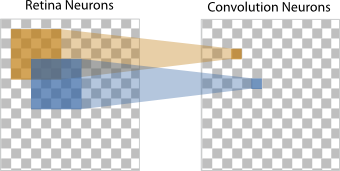
\includegraphics[width=0.6\textwidth]{pics/convolution.png}
	\caption{Each individual convolution neuron connects to its respective field using the same kernel.}
	\label{fig:conv}
\end{figure}

\section{Model Description}
\label{sec:mds}
There are two CNNs proposed to accomplish the posture recognition task.
A straight forward method of template matching was employed at first, and then a multi-layer perceptrons (MLP) was trained to improve the recognition performance.
\subsection{Manual Feature Extraction Model}

\begin{figure}
\centering
	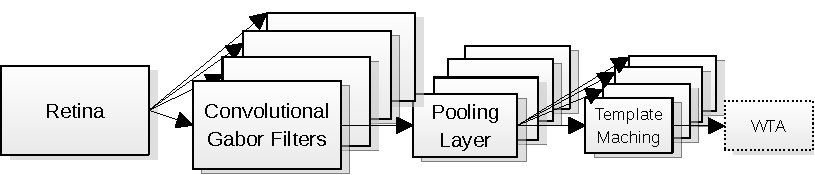
\includegraphics[width=0.7\textwidth]{pics/model1.pdf}
	\caption{The convolutional neural network model with manually selected templates.}
	\label{fig:model1}
\end{figure}

Shown in Figure~\ref{fig:model1} the first two layers are the input layer and the convolution layer, where the kernels are Gabor filters responding to four orientations. 
The third layer is the pooling layer where the size of the populations shrinks. 
This down-sampling enables robust classification due to its tolerance to variations in the precise shape of the input. 
The fourth layer is another convolution layer where the output from the pooling layer is convolved with the templates. 
Each template is a “frame” (one frame consists of 30ms of spiking activity) of output spikes from the pooling layer.
The Gabor filter is well-known as a linear filter for edge detection in image processing. 
A Gabor filter is a 2D convolution of a Gaussian kernel function and a sinusoidal plane wave; see Equation~\ref{equ:gabor}. 
$\theta$ represents the orientation of the filter, $\lambda$ is the wavelength of the sine wave, and $\sigma$ is the standard deviation of the Gaussian envelope. 
The frequency and orientation features are similar to the responses of V1 neurons in the human visual system. 
Only the real parts of the Gabor filters (see Figure~\ref{fig:gabor}) are used as the convolutional kernels to configure the weights between the input layer and the Gabor filter layer.

\begin{equation}
\begin{array}{l}
Real Parts = \exp (\frac{-x^{'2}+y^{'2}}{2\sigma ^{2}})\cos (2\pi\frac{{x}'}{\lambda })
\\
\\
Imaginary Parts = \exp (\frac{-x^{'2}+y^{'2}}{2\sigma ^{2}})\sin (2\pi\frac{{x}'}{\lambda })
\\
\\
where:
\\
\\
{x}'=x\cos (\theta ) + y\sin (\theta)
\\
\\
{y}'=-x\sin (\theta ) + y\cos (\theta)
\end{array}
\label{equ:gabor}
\end{equation}


\begin{figure}
\centering
	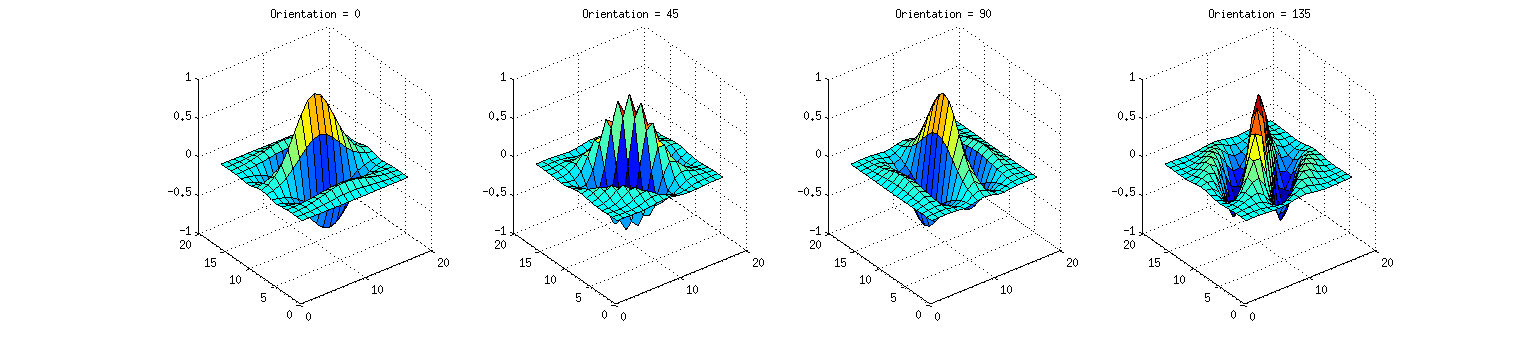
\includegraphics[width=0.95\textwidth]{pics/gabor.png}
	\caption{Real parts of the Gabor filters oriented to four directions.}
	\label{fig:gabor}
\end{figure}

The templates (see Figure~\ref{fig:template}) are manually selected from the output of the pooling layer in the framed Matlab simulation. 
The output score of a convolution neuron is higher when its receptive field matches a certain template more. 
There are five populations of template matching neurons for five gestures in our system. 
The activity of the template matching populations indicates naturally the position of the gestures.

\begin{figure}
\centering
	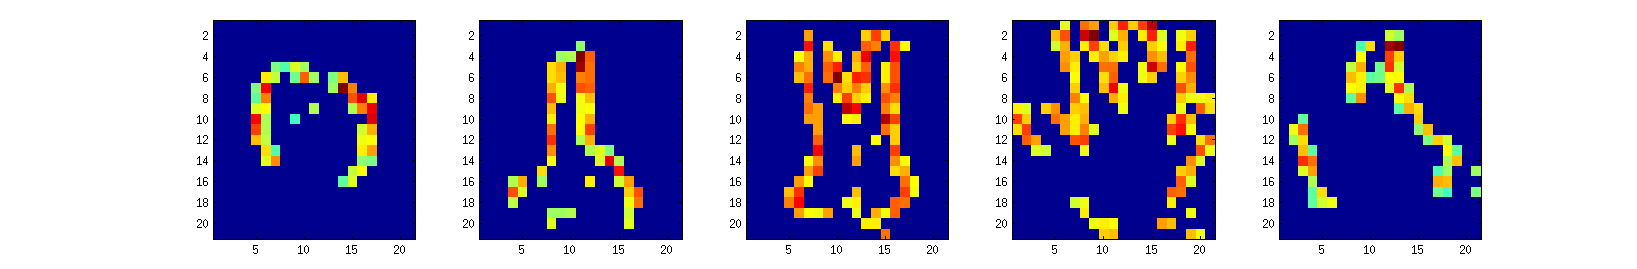
\includegraphics[width=0.95\textwidth]{pics/guesture.png}
	\caption{Five gesture templates}
	\label{fig:template}
\end{figure}

\textcolor{red}{Biology background on V1, especially for Gabor Filters.}

\subsection{Combined Convolution Network}
Inspired by the research of Lecun~\cite{lecun1998gradient} and etc., we designed a combined network model with MLP and the convolutional network (Figure~\ref{fig:model2}). 
Thanks to the help of tracking, only the most active region in the pooling layer is forwarded to the next layer. 
A trained static 3-layered MLP is attached to classify the gesture.

\begin{figure}
\centering
	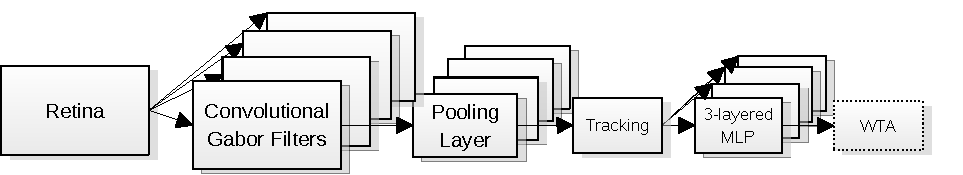
\includegraphics[width=0.8\textwidth]{pics/model2.pdf}
	\caption{The combined convolutional model with trained MLP neurons.}
	\label{fig:model2}
\end{figure}

Since the size of the input image of the MLP training is fixed and the position is centered, tracking plays a very important role to spot the valid region. 
Tracking is naturally embedded in the pooling layer of the convolutional network, for the active neurons directly point out the lively receptive field. 
\textcolor{red}{However, to extract only the active region to the next layer is still need to investigate.}

\section{Training and test}
\label{sec:tat}

Training is missing here.

In order to evaluate the cost and performance trade-offs in optimizing the number of neural components, both the convolutional models described above were tested at different sizes. 
Five gesture videos were captured from the silicon retina in address-event representation (AER~\cite{lazzaro1995multi}) format.  
All the gestures are of similar size and moving clock-wise in front of the retina. 
The videos are cut into frames (30ms/frame) and push forward into the convolutional networks. 
The configurations of the networks are listed in Table~\ref{tbl:nns} (Model 1: template matching; Model 2: trained MLP). 
The integration layer is not necessary in a convolutional network, it is used here to fit the template matching and decrease the number of synaptic connections.

\begin{table}
\caption{Sizes of the convolutional neural networks.}
	\begin{subtable}{1\textwidth}
		
		\centering
		\caption{Model 1: Template matching}
		\begin{tabular}{p{0.16\textwidth}|p{0.16\textwidth}<{\centering}|p{0.16\textwidth}<{\centering}|p{0.16\textwidth}<{\centering}|p{0.16\textwidth}<{\centering}}
		%Line 1
		\Xhline{1.2pt}
		    & \multicolumn{2}{c|}{\tabincell{c}{\textbf{Full} \\\textbf{Resolution}}}  
		    & \multicolumn{2}{c}{\tabincell{c}{\textbf{Sub-sampled} \\\textbf{Resolution}}}
		    \\ \cline{2-5}
		%Line 2
			& \tabincell{c}{Neuron \\ Number}
			& \tabincell{c}{Connections \\ per Neuron}
			& \tabincell{c}{Neuron \\ Number}
			& \tabincell{c}{Connections \\ per Neuron}
			\\ \Xhline{1.2pt}
		%Line 3
		\tabincell{l}{\textbf{Retinal} \\\textbf{Input}}
			& 128 $\times$ 128	& 1	& 32 $\times$ 32	& 4 $\times$ 4
			\\ \hline
		%Line 4
		\tabincell{l}{\textbf{Gabor} \\\textbf{Filter}}
			& 112$\times$112$\times$4	& 17 $\times$ 17	& 28$\times$28$\times$4	& 5 $\times$ 5
			\\ \hline
		%Line 5
		\tabincell{l}{\textbf{Pooling} \\\textbf{Layer}}
			& 36$\times$36$\times$4	& 5 $\times$ 5	& null	& null
			\\ \hline
		%Line 6
		\tabincell{l}{\textcolor[rgb]{0.55,0.55,0.55}{\textbf{Integration}} \\ \textcolor[rgb]{0.55,0.55,0.55}{\textbf{Layer}}}
			& 36 $\times$ 36	& 4	& 28 $\times$ 28	& 4
			\\ \hline
		%Line 7
		\tabincell{l}{\textbf{Template} \\\textbf{Matching}}
			& 16$\times$16$\times$5	& 21 $\times$ 21	& 14$\times$14$\times$5	& 15 $\times$ 15
			\\ \Xhline{1.2 pt}
		%Line 8
		\textbf{Total}
			& $74\,320$	& $15\,216\,512$	& $5\,925$	& $318\,420$
			\\ \Xhline{1.2 pt}
		\end{tabular}
		\label{tbl:m1}
	\end{subtable}
	\par\bigskip
	\begin{subtable}{1\textwidth}
		
		\centering
		\caption{Model 2: Trained MLP network layers after tracking}
		\begin{tabular}{p{0.16\textwidth}|p{0.16\textwidth}<{\centering}|p{0.16\textwidth}<{\centering}|p{0.16\textwidth}<{\centering}|p{0.16\textwidth}<{\centering}}
		%Line 1
		\Xhline{1.2pt}
		    & \multicolumn{2}{c|}{\tabincell{c}{\textbf{Full} \\\textbf{Resolution}}}  
		    & \multicolumn{2}{c}{\tabincell{c}{\textbf{Sub-sampled} \\\textbf{Resolution}}}
		    \\ \cline{2-5}
		%Line 2
			& \tabincell{c}{Neuron \\ Number}
			& \tabincell{c}{Connections \\ per Neuron}
			& \tabincell{c}{Neuron \\ Number}
			& \tabincell{c}{Connections \\ per Neuron}
			\\ \Xhline{1.2pt}
		%Line 3
		\tabincell{l}{\textbf{Tracked} \\\textbf{Input}}
			& 21 $\times$ 21	& null	& 15 $\times$ 15	& null
			\\ \hline
		%Line 4
		\tabincell{l}{\textbf{Hidden} \\\textbf{Layer}}
			& 10	& 21$\times$21$\times$10	& 10	& 15$\times$15$\times$10
			\\ \hline
		%Line 5
		\tabincell{l}{\textbf{Recognition} \\\textbf{Layer}}
			& 5	& 5$\times$10	& 5	& 5$\times$10
			\\ \Xhline{1.2pt}
		%Line 6
		\textbf{Total}
			& $456$	& $4\,460$	& $240$	& $2\,300$
			\\ \Xhline{1.2 pt}
		\end{tabular}
		\label{tbl:m2}
	\end{subtable}
	\label{tbl:nns}
\end{table}

\section{Experiments}
\label{sec:exp}

\begin{figure}
\centering
	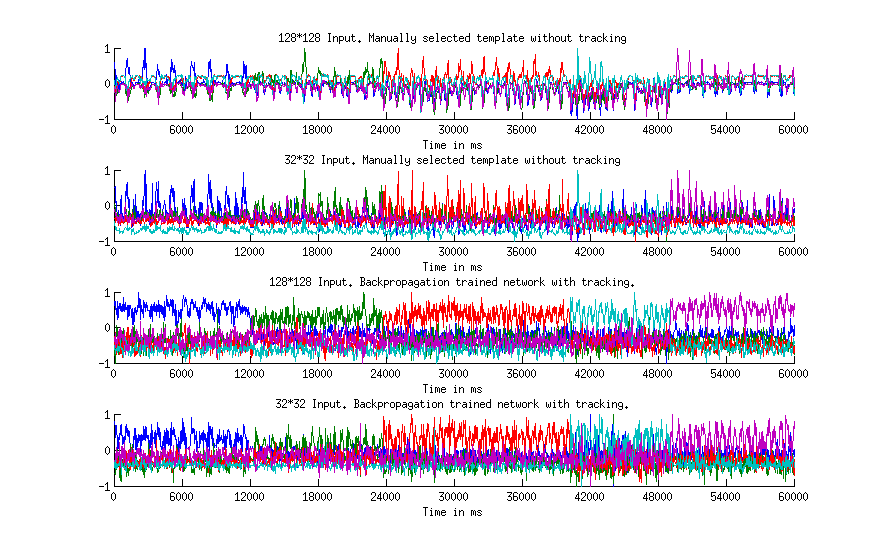
\includegraphics[width=1\textwidth]{pics/4.png}
	\caption{Neuron responses to the same five gesture videos.}
	\label{fig:matlabrec}
\end{figure}




In Figure~\ref{fig:matlabrec} the first two plots refer to Model 1, using template matching. Each colour represents one of the recognition populations. 
Each point in the plot is the highest neuronal response in the recognition population during the time of one frame (30 ms). 
The neuronal response, the spiking rate, is normalized to [-1, 1]. 
It can be seen that the higher resolution input makes the boundaries between the classes clearer. 
On the other hand, recognition only happens when the test image and template are similar enough. 
The templates are only selected from the frames where the gestures are moving towards the right, and the gestures are moving clockwise in the videos. 
Thus, all the peaks in plot 1 signify that the direction of the gestures’ movement is right.  
It is notable that the higher resolution causes the recogniser to be more sensitive to the differences between the test data and the template, while the smaller neural network can recognize more generalized patterns. 
Therefore, a threshold is required to differentiate between data that is close enough and that which is not. 
Since the gestures are moving in four different directions during the clockwise movement, a rejection rate of 75\% is to be expected. 
The latter two plots refer to Model 2. 
The three-layer MLP network significantly improves the recognition rate and can generalize the pattern. 
There is no rejection rate for Model 2. 
The detailed results are listed in  Table~\ref{tbl:rsl}. 
The correct recognition rate is calculated from the non-rejected frames.
The lower resolution of the 32$\times$32 retina input is adequate for this gesture recognition task. 
The smaller network uses only 1/10 the number of neurons and 1/50 the number of synaptic connections compared to the full resolution network, while the recognition rate drops only around 10\% with Model 1 and 15\% with Model 2.

\begin{table}
\centering
\caption{Recognition results}
	\begin{tabular}{p{0.16\textwidth}|p{0.12\textwidth}<{\centering}|p{0.12\textwidth}<{\centering}|p{0.12\textwidth}<{\centering}|p{0.12\textwidth}<{\centering}|p{0.12\textwidth}<{\centering}}
		%Line 1
		\Xhline{1.2pt}
		    \multicolumn{2}{c|}{}	& \multicolumn{2}{c|}{\textbf{Model 1}}  
		    & \multicolumn{2}{c}{\textbf{Model 2}}
		    \\ \cline{3-6}
		%Line 2
		\multicolumn{2}{c|}{}	& \tabincell{c}{High \\ Resolution}
			& \tabincell{c}{Low \\ Resolution}
			& \tabincell{c}{High \\ Resolution}
			& \tabincell{c}{Low \\ Resolution}
			\\ \Xhline{1.2pt}
		%Line 3-4	
		\multirow{2}{*}{\tabincell{l}{\textbf{Fist} \\ (399 Frames)}}
			& Correct & 99.11\%	& 99.23\%	& 96.24\%	& 84.21\%
			\\ \cline{2-6}
			& Reject  & 71.93\% & 67.42\% 	& Null	& Null
			\\ \hline
		%Line 5-6
		\multirow{2}{*}{\tabincell{l}{\textbf{One Finger} \\ (392 Frames)}}
			& Correct & 92.98\%	& 80.00\%	& 94.39\%	& 71.69\%
			\\ \cline{2-6}
			& Reject & 70.92\%	& 75.77\% 	& Null	& Null
			\\ \hline
		%Line 7-8
		\multirow{2}{*}{\tabincell{l}{\textbf{Victory Sign} \\ (551 Frames)}}
			& Correct & 96.56\%	& 93.07\%	& 95.64\%	& 87.66\%
			\\ \cline{2-6}
			& Reject & 73.68\%	& 81.67\% 	& Null	& Null
			\\ \hline
		%Line 9-10
		\multirow{2}{*}{\tabincell{l}{\textbf{Full Hand} \\ (293 Frames)}}
			& Correct & 95.65\%	& 72.41\%	& 93.52\%	& 72.01\%
			\\ \cline{2-6}
			& Reject & 92.15\%	& 90.10\% 	& Null	& Null
			\\ \hline
		%Line 10-11
		\multirow{2}{*}{\tabincell{l}{\textbf{Thumb up} \\ (391 Frames)}}
			& Correct & 89.61\%	& 84.44\%	& 96.68\%	& 74.68\%
			\\ \cline{2-6}
			& Reject & 80.31\%	& 76.98\% 	& Null	& Null
			\\ \hline
	\end{tabular}
	\label{tbl:rsl}
\end{table}